\section{Feature Extraktion bei kontinuierlichen Livedaten}\label{kap:featureextraktion}

Durch die stetige Aufnahme von Sensordaten um Maschinen zu überwachen, entsteht ein kontinuierlicher Datenfluss. 
Wie in den vorherigen Kaptiteln beschrieben, stellt diese Eigenschaft eine hohe Anforderung an Lernalgorithmen. 
Einige Lernalgorithmen verwenden das Konzept des \enquote{Lazy Learnings}, im Deutschen \enquote{träges Lernen}. 
Bei diesen Lernalgorithmen wird das Modell auf Anfrage erstellt. 
Das bedeutet, jede Eingabe startet eine neue Modellbildung und fordert daher in kürzester Zeit eine hohe Rechenleistungen. Beim \enquote{Eeager Learning}, im Deutschen \enquote{Eifriges Lernen}, hingegen wird schon im Vorfeld mithilfe von Trainingsdaten ein Model bereitgestellt. 
Der Ressourcenverbrauch bei einer Anfrage von neuen Daten ist dann sehr gering~\cite{Gay2013}. 

Bei den kontinuierlichen Livedaten in der Maschinenüberwachung stehen die Daten meist auch zeitlich in Korrelation. Daher ist die Rede von Zeitreihendaten. Die Reihenfolge dieser Daten spielt bei der Analyse eine große Rolle. Zeitreihendatensätze werden mathematisch wie in dem Datensatz \ref{equ:trainingset} dargestellt. Eines der Ziele für Lernalgorithmen kann es sein aus dem Datensatz \ref{equ:trainingset} die Daten 

\begin{equation}
  \tau_{n+1}, \tau_{n+2}, ...
  \label{equ:predictionset}
\end{equation}
vorherzusagen.

Das Ziel ist es aus den Daten mittels Analysealgorithmen Informationen über die Maschine zu gewinnen. 
Um dies effizient zu erreichen, können gewissen Merkmale vordefiniert oder extrahiert werden. 
Eine bewerte Methode ist das Zerlegen der Zeitreihendaten.

\subsection{Zeitreihenzerlegung}
Bei der Zeitreihenzerlegung werden die zeitlich korrelierenden Daten durch additive oder multiplikative Verfahren in Merkmale zerlegt. 
Diese können anschließend wieder durch zusammenführen in den Grunddatensatz zurückgeführt werden.
Die zerlegten Datensätze liefern im zerlegten Zustand jeweils eine spezielle Information, basierend auf der Art der Zerlegung.

\subsubsection{Zerlegung in Trend und Saisonkomponente}
Bei der Zerlegung von Zeitreihen in Trend- und Saisonkomponenten wird die Zeitreihe typischerweise in folgende Komponenten aufgeteilt~\cite{Leonard2018}:
\begin{itemize}
  \item $T_t$ Trendkomponente, stellt den langfristigen Verlauf dar.
  \item $C_t$ Zykluskomponente, stellt wiederholte Schwankungen dar.
  \item $S_t$ Saisonkomponente, stellt Schwankungen in festen und bekannten Zeiträumen dar.
  \item $I_t$ unregelmäßige Komponente, stellt unregelmäßige Schwankungen dar.
\end{itemize}
Dabei werden Trend- und Zykluskomponenten gerne zu einer Trendzykluskomponente zusammengefasst.



\begin{figure}
  \centering
  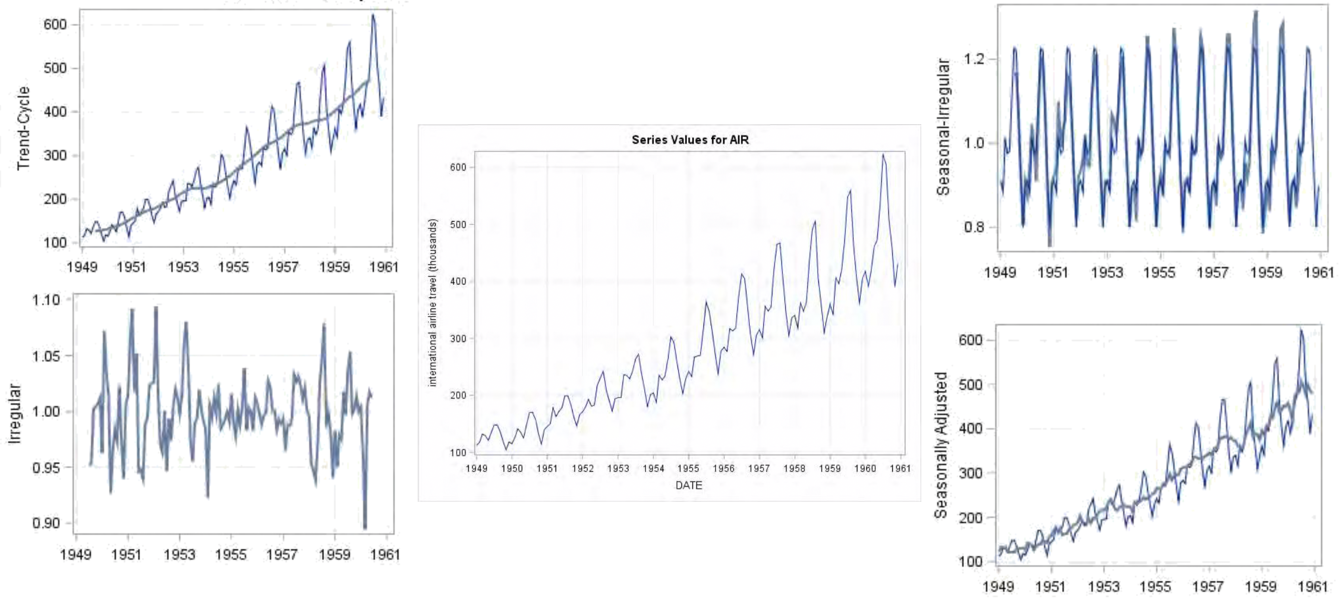
\includegraphics[width=1\textwidth]{trendsaisondecomposition.png}
  \caption{Zeitreihenzerlegung anhand des \enquote{Sashelp.Air} Datensatz. Dieser wurde durch die Komponenten TrendZyklus (Trend-Cycle), Saisonal unregelmäßige (Seasonal-Irregular), Saisonal (Seasonally/Adjusted) und unregelmäßige (Irregular) dargestellt~\cite{Leonard2018}. }
  \label{fig:trendsaisondecomposition}
\end{figure}

Der Informationsgewinn dieser Aufteilung wird durch das Praxisbeispiel aus Abbildung\ \ref{fig:trendsaisondecomposition} deutlich. 
Es werden die internationalen Fluggastdaten aus dem \enquote{Sashelp.Air} Datensatz in einer Zeitreihe dargestellt. Für jeden Monat ist die Gesamtanzahl an grenzüberschreitende Fahrgästen zu sehen. 
Der Datensatz wurde anschließend in:
\begin{itemize}
  \item Trendzyklus Komponente (oben links)
  \item Saisonal unregelmäßige Komponente (oben Rechts)
  \item Unregelmäßige Komponente (unten links)
  \item Saisonale Komponente (unten rechts)
\end{itemize}
aufgeteilt. 
Durch die Trendzyklus Komponente ist ein deutlicher Anstieg zwischen den Jahren 1949 und 1961 erkennbar. 
Die Saisonkomponenten lassen darauf schließen, dass die Anzahl der grenzüberschreitenden Fluggäste stark von den Jahreszeiten abhängen~\cite{Leonard2018}. 

Durch die Zeitreihenzerlegung werden Informationen durch Fokussieren verschiedener Metriken leichter extrahiert. Zudem wird die Komplexität um die jeweiligen Komponenten weiter zu Analysieren stark reduziert. Dennoch ist die Verarbeitung und Visualisierung großer Zeitreihen sehr aufwändig bei dieser Methode.

\subsection{Motivfindung}
Im Gegensatz zu der Zeitreihenzerlegung ist die Idee bei der Motivfindung nicht, die Zeitreihen in Komponenten zu zerlegen, sondern es wird versucht Motive in den Zeitreihen zu identifizieren.
Motive sind nach ihrer Identifizierung verwendbare Merkmale als Eingabe für Lernalgorithmen. Zur Motividentifizierung gibt es unterschiedliche Ansätze:
\begin{itemize}
  \item \enquote{brute-force} basiert
  \item Probabilistische Methoden als Basis
  \item Eine Motivbewertung, welche Motivinstanzen in einer Zielinstanz ausfindig macht
  \item Anomaliedetektion in Teilsequenzen
\end{itemize}

Durch alle diese Ansätze werden die stellen eines Motivs in einer Zeitreihe identifiziert~\cite{Leonard2018}. 
\begin{figure}
  \centering
  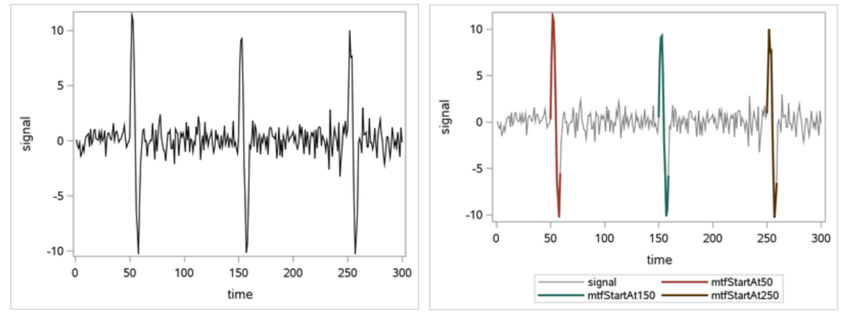
\includegraphics[width=0.8\textwidth]{motifdiscovery.png}
  \caption{Darstellung der in einer Zeitreihe identifizierten Motive~\cite{Leonard2018}. }
  \label{fig:motivdiscovery}
\end{figure}

In Abbildung\ \ref{fig:motivdiscovery} wurde anhand von einem \enquote{brute-force} Ansatz drei Motive in einem Zeitreihendatensatz erkannt.
Je mehr Motive gefunden werden, desto genauer können die Lernalgorithmen die Daten anhand der Motive unterscheiden.
Es wird aber auch komplizierter die Analyse durchzuführen~\cite{Leonard2018}.

Daher ist es auch immer ein Ziel. Die Anzahl an Merkmalen zu reduzieren. 
Um Zeitreihendatensätze zu reduzieren wird die Dimension entstehend durch Parameter oder extrahierten Merkmalen versucht möglichst auf die Notwendigen zu reduzieren. Zeitreihendaten aus Sensoren sind oft hoch korrelierend, was zu einer sehr großen Datenredundanz führt. 
Eine bewerte Technik um Datenmengen aus Sensordaten fester Größe darzustellen ist die \enquote{Fourier Transforamtion}. 

\subsection{Parametrisierung durch die Fourier Transformation}

Bei der Fourier Transformation werden die Signale auf einen Frequenzbereich abgebildet und diese Abbildung mittels Koeffizienten dargestellt. Da es sich bei den kontinuierlichen Sensordaten meist um keinen vollständigen Datenbestand handelt, sondern nur um Datenauszüge, bietet sich die \enquote{Diskrete Fourier Transformation} an.


\begin{equation}
  F_j = \frac{1}{N} \sum_{k=0}^{N-1} f_k W_N^{-kj}  \text{\ \ mit \ \ } W_N = e^{\frac{2\pi i}{N}}
  \label{equ:fourier}
\end{equation}

\begin{equation}
  F_j = \frac{1}{N} (\alpha_0+\alpha_1*e^{i2\pi \frac{t-t_0}{T}}+ \alpha_2*e^{2i2\pi \frac{t-t_0}{T}} + ...)
  \label{equ:fourier}
\end{equation}

Durch die Diskrete Fourier Transformation in Formel\ \ref{equ:fourier} wird der Zeitreihenabschnitt in einer periodische Funktion durch Koeffizienten dargestellt~\cite{Butz2012}. Um die zu analysierenden Merkmale zu reduzieren ist die Idee, dass nicht alle Koeffizienten als Parameter verwenden werden, sondern nur eine Auswahl von diesen. Bekannte Methoden sind dabei entweder die ersten $k$ Koeffizienten zu verwenden. Man speichert quasi nur eine grobe Skizze der Kurven ab. Die ersten Koeffizienten abzuspeichern, behält die tieferen Frequenzen und ist eine sehr naive Herangehensweise. Eine deutlich bessere Methode wäre es die größten Koeffizienten zu verwenden. Diese sind aber sehr aufwändig zu berechnen~\cite{morchen2003time}. Fabian Mörchen stellt dagegen eine Methode in seiner Arbeit \enquote{Time series feature extraction for data mining using DWT and DFT} vor, in der er eine Aggregatsfunktion verwendet, welche die Bedeutung der Koeffizienten misst. Es ist dadurch möglich mit seiner Aggregatsfunktion:

\begin{equation}
  J_k^1(mean(c_j^2), C)
  \label{equ:aggregatefunction}
\end{equation}

eine definierte Menge $k$ an Koeffizienten als Merkmale für Lernalgorithmen als Eingabe zu geben. $k$ entspricht dann der Dimension der zu verarbeitenden Datenmenge. 

\subsection{Extraktion durch Clustern}

Eine weitere Arbeit von Dominique Gay et al. \enquote{Feature Extraction over Multiple Representations for Time Series Calssification} stellt ein Verfahren vor in dem sie Zeitreihendaten so vorverarbeiten, dass in dem Verfahren extrahierte Merkmale die neuen Parameter fester Größe bilden. Dies geschieht in einem Dreischrittverfahren:

\begin{enumerate}
  \item Der Datensatz wird in mehrere Datenrepräsentationen transformiert
  \item Auf jede Repräsentation wird ein Co-Clustering Verfahren angewendet
  \item Aus jeder Repräsentation wird eine Menge an Merkmalen erstellt und daraus ein neuer Datensatz generiert
\end{enumerate}

Für den ersten Schritt schlagen sie verschiedene Transformationsverfahren vor. Beispielsweise Ableitungen oder kumulatives Integrieren. In einem Beispiel sind die Vorteile einer solchen Vorverarbeitung erkennbar. In Abbildung\ \ref{fig:derivative} ist in (a) ein Zweiklassen \enquote{ARSim} Datensatz zu sehen. Dieser ist unverarbeitet und die Klassen sind farblich Markiert. Die Klassen sind in (a) nur sehr schwer separierbar. In (b) wurde der selbe Datensatz durch zweifaches Ableiten transformiert und wieder in einem Datenplot und farblicher Markierung dargestellt. Durch die Transformation sind die Klassen schon deutlicher erkennbar.

\begin{figure}
  \centering
  \includegraphics[width=1\textwidth]{plotAbleitung.png}
  \caption{In (a) ein unverarbeiteter original geplotteter Datensatz und in (b) der gleiche durch zweifache Ableitungen transformierter Datensatz~\cite{Gay2013}.}
  \label{fig:derivative}
\end{figure}

Der transformierte Datensatz bilde somit eine bessere Grundlage um mithilfe von Klassifizierungsalgorithmen die Daten zu Differenzieren. 
Der zweite Schritt ist das Co-Clustering. 
Dabei wird das Clustering als eine Vorverarbeitung für nachfolgende Lernalgorithmen verwendet. 
Die Idee ist es ähnliche Daten zu gruppieren und lokale Muster hervorzuheben~\cite{gay2013feature}. Dabei stellen sie die Kurven in einer Menge $(X,Y)$ dar und fügen jeder dieser Mengen eine Klasse $Cid$ hinzu um sie der jeweiligen Kurve zuzuordnen. Es entsteht eine dreidimensionale Darstellung der Punkte. Das Ganze wird in eine dreidimensionale Gitterstruktur gebracht. Das Endziel ist es Kurven- und Intervallcluster zu erhalten die Anschließend als Merkmalsgrundlage dienen. 

Erreicht wird das durch das Anwenden des \enquote{Khiops Coclustering}\cite{boulle2012functional}. Dabei wird das optimale Gitterfeld durch die Optimierung des Bayes'schen Kriteriums, der sogenannten Kosten ermittelt. 
\begin{equation}
  cost(M) = -log(p(M) \times p(D|M))
  \label{equ:Bayesian}
\end{equation}
Als Resultat lassen sich die Kosten so interpretieren, dass bei niedrigen Kosten eine hohe Kompression der Daten $D$ auf das Modell $M$ herrscht. Wobei das Modell in diesem Fall das optimale Gitterfeld ist.

\begin{figure}
  \centering
  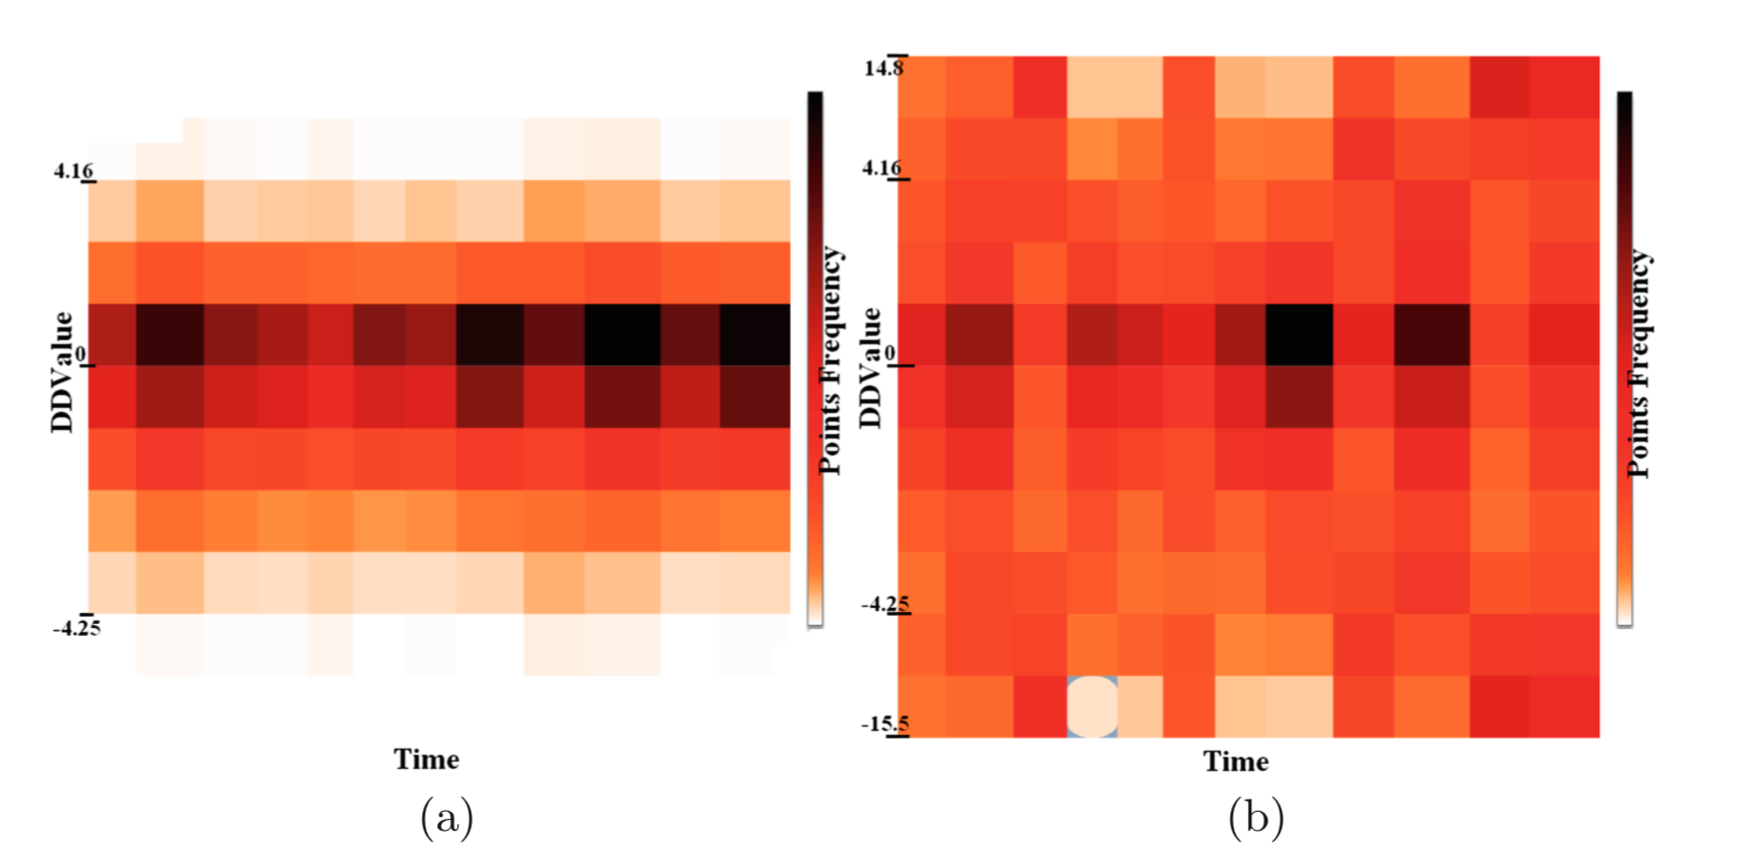
\includegraphics[width=1\textwidth]{coclustering.png}
  \caption{Ergebnis eines Co-Clustering mit \enquote{Khiops Coclustering}~\cite{Gay2013}.}
  \label{fig:coclustering}
\end{figure}

Ein durchgeführtes Co-Clustering ist in Abbildung\ \ref{fig:coclustering} zu sehen. Dabei ist die dritte Dimension Farblich dargestellt. Als Ergebnis sind 25 Cluster von Kurven entstanden. 

Als letzte Schritte müssen noch die Merkmale extrahiert und ein Datensatz generiert werden. Es werden drei Merkmale definiert:

\begin{enumerate}
  \item $K_C$ ein numerisches Merkmal, welches die Unähnlichkeitswahrscheinlichkeit zu allen Kurvenclustern angibt.
  \item Ein kategorisches Merkmal als Index, welcher das nächste Kurvencluster angibt.
  \item $K_Y$ ein numerisches Merkmal, welches die Anzahl an Punkten dieser Kurve in der jeweiligen Klasse angibt.
\end{enumerate}

Durch dieses Verfahren wird die Dimension der Livedaten mit Hilfe von \enquote{Feature Extraktion} auf Drei festgelegt und kann somit durch \enquote{Eager Learning} Algorithmen analysiert werden.

\subsection{Ähnlichkeitsanalyse}
Bei der Ähnlichkeitsanalyse wird der Unterschied unter Berücksichtigung der Ordnung zwischen Eingabe- und Zielsequenz gemessen. 
Zusätzlich können diese Verfahren auch die Zielsequenz in Richtung der Eingabesequenz verschieben um möglichst effizient die Ähnlichkeit zu messen~\cite{Leonard2018}. 
In Abbildung\ \ref{fig:similarityanalysis} ist eine solche Verschiebung durch ein Ähnlichkeitsmaß abgebildet. 
Dabei wird die Zielsequenz im oberen rechten Bild auf die Eingabesequenz im oberen linken Bild verschoben. Die Verschiebung und Ähnlichkeit ist in dem Bild unten Rechts dargestellt.
\begin{figure}
  \centering
  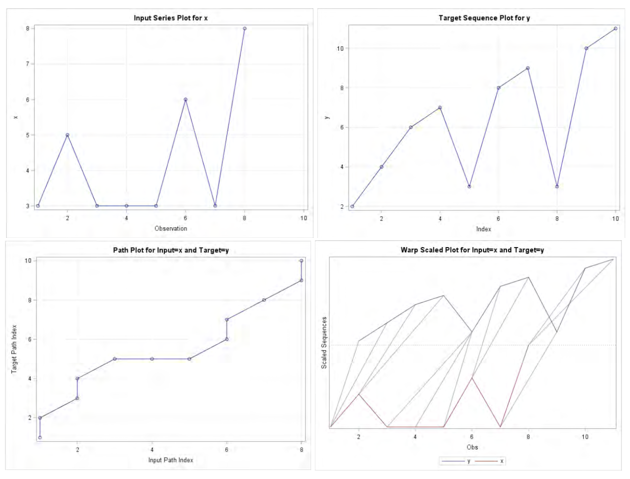
\includegraphics[width=0.8\textwidth]{similarityanalysis.png}
  \caption{Darstellung einer Ähnlichkeitsanalyse auf Basis einer Datenverschiebung. Oben links die Eingangssequenz wird wie in der Abbildung unten rechts auf die Zielsequenz oben rechts verschoben~\cite{Leonard2018}.}
  \label{fig:similarityanalysis}
\end{figure}

Dieses Ähnlichkeitsmaß stellt ein Merkmal da anhand dessen Sensordaten in Form von Zeitreihendaten verglichen werden können. 
Durch die Ähnlichkeitsanalyse können auch mehrere Sequenzen miteinander verglichen werden und daraus eine Ähnlichkeitsmatrix erstellt werden.